\documentclass[11pt]{beamer}
\usetheme{CambridgeUS}
\usepackage[utf8]{inputenc}
\usepackage{amsmath}
\usepackage{amsfonts}
\usepackage{amssymb}
\usepackage[
backend=biber,
style=alphabetic,
citestyle=authoryear
]{biblatex}
\usepackage{array}
\usepackage{xcolor}

% Footnote without number
\newcommand\blfootnote[1]{%
  \begingroup
  \renewcommand\thefootnote{}\footnote{#1}%
  \addtocounter{footnote}{-1}%
  \endgroup
}
\def\boxit#1{%
  \smash{\color{red}\fboxrule=1pt\relax\fboxsep=2pt\relax%
  \llap{\rlap{\fbox{\vphantom{0}\makebox[#1]{}}}~}}\ignorespaces
}
\addbibresource{stats.bib}
\title[Bioestatística II] %optional
{Teste t de amostras relacionadas}

\subtitle{CGF2046 - Bioestatística II}

\author[da Silva, Ricardo] % (optional, for multiple authors)
{R. ~R. ~da Silva\inst{1}}

\institute[FCFRP] % (optional)
{
  \inst{1}%
  Departamento de Ciências BioMoleculares\\
  Faculdade de Ciências Farmacêuticas

}

\date{\today} % (optional)

\titlegraphic{
\includegraphics[width=5.8cm]{figs/logo_final}} 

\begin{document}

%\begin{frame}
%\titlepage
%\end{frame}

%\begin{frame}
%\tableofcontents
%\end{frame}

\begin{frame}
\titlepage
\end{frame}

\begin{frame}
\label{contents}
\frametitle{Sumário}
\tableofcontents
\end{frame}

\setbeamercovered{transparent}
\begin{frame}
\frametitle{Objetivos de Aprendizado\footcite{carlson2017introduction}}
  Depois de assitir essa aula e fazer as atividades complementares, você será capaz de:
  \\~\\
  \begin{itemize}
  \uncover<1->{\item
    Identificar quando um teste t de amostras relacionadas deve ser usado;}
  \uncover<2->{\item
    Explicar as vantagens de usar um desenho de amostras relacionadas em vez de um desenho de amostras independentes;}
   \uncover<3->{\item
    Explicar a lógica do teste t de amostras relacionadas;}
   \uncover<4->{\item
    Escrever hipóteses nulas e de pesquisa usando símbolos e palavras para testes unicaudais e bicaudais;}
   \uncover<5->{\item
    Calcular um teste t de amostras relacionado manualmente (usando uma calculadora) e usando \textit{software};}
   \uncover<6->{\item
    Determinar se você deve ou não rejeitar a hipótese nula;}
   \uncover<7->{\item
    Calcular e interpretar um tamanho de efeito (d);}
   \uncover<8->{\item
    Resumir os resultados da análise.}            
  \end{itemize}
\end{frame}

\section{Introdução ao teste t}
\setbeamercovered{transparent}
\begin{frame}
\frametitle{Amostras Repetidas/Relacionadas}
Embora seu cálculo seja semelhante ao teste t para amostra única, esse novo teste t tem vários nomes diferentes, um para cada projeto experimental em que pode ser usado. 

Exemplos:
\begin{itemize}
\item \textit{teste t de medidas repetidas}: comparar a média de uma amostra de pessoas antes e depois de receberem um tratamento;
\item \textit{teste t de amostras relacionadas}: comparar dois grupos de participantes que estão relacionados de alguma forma;
\item também é às vezes chamado de teste t de amostras pareadas, teste t de amostras combinadas, teste t de amostras dependentes ou teste t dentro dos sujeitos.
\end{itemize}

\end{frame}

\setbeamercovered{transparent}
\begin{frame}
\frametitle{Amostras Repetidas/Relacionadas}
Por exemplo, se os investigadores quisessem testar a eficácia de um novo medicamento destinado a reduzir a ansiedade, poderiam recolher uma amostra de pessoas, medir primeiro a sua ansiedade, depois administrar-lhes o novo medicamento e, finalmente, medir a sua ansiedade depois de o medicamento ter tido tempo de fazer efeito.\\~\\

Se for improvável que o desvio entre as duas médias amostrais seja criado por erro amostral, então presume-se que o medicamento tenha alterado o nível de ansiedade da amostra.

\end{frame}

\setbeamercovered{transparent}
\begin{frame}
\frametitle{Lógica do Testes t de Amostra Única e Amostras Repetidas/Relacionadas}
A lógica do teste t de amostras relacionadas é semelhante à do teste t de amostra única.\\~\\

t Amostra única = $\frac{(\bar{x} - \mu)}{SEM_a}$\\~\\

t Amostra repetidas/relacionadas = $\frac{(\bar{x}_D - \mu_D)}{SEM_D}$\\~\\

O numerador do teste t de amostras relacionadas compara a diferença média entre duas médias amostrais com a diferença média esperada se o nulo for verdadeiro. Se você usar $\mu_D = 0$\\~\\

t Amostra repetidas/relacionadas = $\frac{\bar{x}_D}{SEM_r}$\\~\\

Se o valor t obtido estivesse mais distante de 0 que o valor crítico, a hipótese nula seria rejeitada.

\end{frame}

\setbeamercovered{transparent}
\begin{frame}
\frametitle{Teste t unicaudal de amostra única}

\textbf{Exemplo:} Um pesquisador clínico quer determinar se um novo medicamento para tratar a ansiedade tem efeitos colaterais que alteram os níveis de colesterol. 
 
\begin{itemize}
\item Os níveis de colesterol são normalmente distribuídos e medidos como uma variável quantitativa;
\item
   Seis pares de pessoas são comparadas em relação aos seus níveis de colesterol pré-existentes. Em seguida, uma pessoa de cada par recebe o novo medicamento para ansiedade, enquanto a outra pessoa recebe um placebo;
\item
  Dezoito semanas depois, o pesquisador mede os níveis de colesterol.
\end{itemize}

Optamos por um teste bilateral. Também escolhemos um \(\alpha=0.05\).

\end{frame}

\setbeamercovered{transparent}
\begin{frame}
\frametitle{Etapa 1: examinar as pressuposições estatísticas}

Todos os testes de hipóteses são baseados em suposições específicas e, se essas suposições forem violadas, esses testes podem produzir resultados enganosos.\\~\\
Os quatro pressupostos básicos são:

\begin{enumerate}
\item independência dos dados;
\item medição apropriada das variáveis para análise;
\item normalidade das distribuições.
\end{enumerate}

\end{frame}

\setbeamercovered{transparent}
\begin{frame}
\frametitle{Etapa 1: examinar as pressuposições estatísticas}

Os três pressupostos básicos são:

\begin{enumerate}
\item \textbf{independência dos dados:} A VI neste estudo identifica dois grupos relacionados, designados aleatoriamente para duas condições diferentes;
\item \textbf{medição apropriada:} variável independente (VI) \(\Rightarrow\) identifica as duas condições de medicamento versus placebo, variável dependente (VD) \(\Rightarrow\) nível de colesterol dos participantes, é medido em como uma variável quantitativa;
\item \textbf{normalidade das distribuições:} população original de diferenças médias é normalmente distribuida.
\end{enumerate}

\end{frame}

\setbeamercovered{transparent}
\begin{frame}
\frametitle{Etapa 2: expor as hipóteses nulas e de pesquisa simbolicamente e verbalmente}

O teste t de amostras relacionadas determina se a média dessas diferenças é significativamente diferente de 0.

\begin{center}
\begin{tabular}{ m{2cm}|m{2cm}|m{3cm}|m{3cm} } 
 \hline
 Tipo de Hipótese & Simbólico & Vebal & Diferença entre médias amostral e populacional\\
  \hline
 Hipótese nula & $\mu_{D}=0;$ & Diferença média $\approx$ 0 & Erro amostral \\ 
 Hipótese de pesquisa & $\mu_{D} \neq 0.$ & Diferença média $\neq$ 0 & Medicamento tem efeito sobre colesterol  \\ 
 \hline
 \hline
\end{tabular}
\end{center}

\end{frame}

\begin{frame}
\frametitle{Etapa 3: Use o tamanho da amostra para calcular os graus de liberdade e defina as regiões críticas}
Depois de saber o tamanho da amostra de um estudo, você precisa calcular seus graus de liberdade (gl). Para o teste t de amostra única, a fórmula para o gl é \textit{gl = N - 1}. Portanto, neste caso,
\[gl = 6 - 1 = 5\]

\begin{columns}
\begin{column}{0.5\textwidth}
   Excerto da tabela t bilateral\\~\\

\begin{center}
\begin{tabular}{ccc} 
 \hline
gl & $\alpha = .05$ & $\alpha = .01$\\
4 &	2.776400 & 4.604100\\
\boxit{1.7in} 5 & 2.570600 & 4.032100\\
6 & 2.446900 & 3.707400\\
 \hline
\end{tabular}
\end{center}   
   
   
\end{column}
\begin{column}{0.5\textwidth}  %%<--- here
   \begin{itemize}
   \item O valor de corte de \(\alpha= .05\) define a região crítica, os valores t são improváveis se o valor nulo for verdadeiro.
   \end{itemize}
\end{column}
\end{columns}
\end{frame}

\setbeamercovered{transparent}
\begin{frame}
\frametitle{Etapa 4: calcular a estatística do teste (teste t de amostras relacionadas)}
\textit{4a. Calcule D para cada participante/par correspondente}\\~\\

A primeira etapa no cálculo da estatística t das amostras relacionadas é calcular o valor da diferença (ou seja, D) para cada par de valores. 

\begin{center}
\begin{tabular}{cccc} 
 \hline
Par & Placebo & Medicamento & D (Medicamento - Placebo)\\
 \hline
A & 180 & 188 & 8 \\
B & 200 & 201 & 1 \\
C & 190 & 197 & 7 \\
D & 170 & 174 & 4 \\
E & 210 & 215 & 5 \\
F & 195 & 194 & -1 \\
 \hline
\end{tabular}
\end{center}   

\end{frame}

\setbeamercovered{transparent}
\begin{frame}
\frametitle{Etapa 4: calcular a estatística do teste (teste t de amostras relacionadas)}
\begin{itemize}
\item 4b. Calcule a diferença média observada ($\bar{x}_D$)

\[\bar{x}_D = \frac{\sum_{i=1}^n D_i}{N} = \frac{24}{6} = 4\]

\item 4c. Calcule a diferença média esperada devido ao erro de amostragem
\[SQ_D = \frac{1}{N-1}\sum_{i=1}^n(D_i - \bar{x}_D)^2 = 12\]
\[SEM_r = \frac{DP}{\sqrt{N}} = \frac{3.464}{\sqrt{6}} = 1.414\]
\item 4d. Calcule a estatística do teste (teste t de amostras relacionadas)
\[t =  \frac{\bar{x}_D}{SEM_r}  = \frac{4}{1.414} = 2.83\]
\end{itemize}
\end{frame}

\setbeamercovered{transparent}
\begin{frame}
\frametitle{Etapa 4: calcular a estatística do teste (teste t de amostras relacionadas)}
O valor t obtido de 2.83 está mais distante de 0 do que o valor crítico de +2.5706.
\begin{center}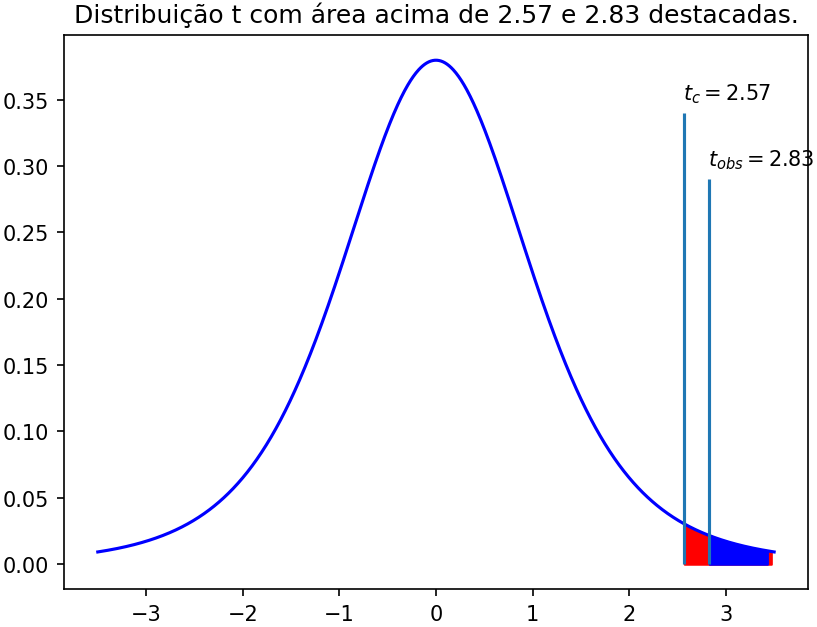
\includegraphics[width=0.55\linewidth]{figs/regiao_critica_observada_t_rel} \end{center}

\end{frame}


\setbeamercovered{transparent}
\begin{frame}
\frametitle{Etapa 5: calcule o tamanho do efeito e descreva se o seu grau}
Um tamanho de efeito é um índice da diferença entre a média da amostra e a média da população. A estatística de tamanho do efeito normalmente usada ao comparar duas médias é d. 
\begin{align*}
d &= \frac{Desvio\quad observado\quad entre\quad as\quad medias}{Desvio\quad padrao}\\
  &= \frac{\bar{x}_D}{DP_D} = \frac{4}{3.464} = 1.15
\end{align*}

\end{frame}

\setbeamercovered{transparent}
\begin{frame}
\frametitle{Etapa 5: calcule o tamanho do efeito e descreva se o seu grau}
A melhor maneira de interpretar qualquer tamanho de efeito é compará-lo com os tamanhos de efeito produzidos por estudos semelhantes na literatura de pesquisa. Se você não conseguir encontrar estudos semelhantes na literatura para fornecer uma referência, poderá usar as diretrizes gerais sugeridas por Cohen (1992) para interpretar os tamanhos dos efeitos na Tabela 6.2.

\begin{center}
\begin{tabular}{cc} 
 \hline
d  & Tamanho estimado do efeito\\
 \hline
Perto de 0.2 & Pequeno \\
Perto de 0.5 & Médio \\
Perto de 0.8 & Grande \\
 \hline
\end{tabular}
\end{center}   

\end{frame}

\setbeamercovered{transparent}
\begin{frame}
\frametitle{Etapa 6: Interpretando os Resultados do Teste de Hipóteses}

As frases a seguir resumem os resultados deste teste t de amostras relacionadas. Você precisará calcular as médias para os grupos de medicamento e placebo manualmente ou usando \textit{software} para incluí-los em seu relatório de resultados.\\~\\

As pessoas que tomaram o ansiolítico apresentaram níveis de colesterol substancialmente mais elevados (\(\bar{x}_A = 194.83\), DP = 13.64) do que as pessoas que tomaram o placebo (\(\bar{x}_P = 190.83\), DP = 14.29), \(t_{(5)} = 2.83\), \(p < 0.05\), d = 1.15. A droga aumentou os níveis de colesterol em mais de 1 desvio padrão, sugerindo que a droga tem um efeito prejudicial sobre os níveis de colesterol. No entanto, a amostra incluiu apenas seis pares de pessoas e, portanto, o estudo deve ser replicado com uma amostra maior.
\end{frame}

\begin{frame}
\frametitle{Exemplo de teste t de amostras relacionadas (unicaudal)}
\textbf{Exemplo:} Um psiquiatra recruta seis pessoas com altos índices de ansiedade para um estudo de avaliação do novo medicamento. Todos os seis voluntários completam um inventário de ansiedade antes de tomar o medicamento e novamente após tomar o medicamento por 1 mês.\\~\\ 

Espera-se que diminua os índices de ansiedade das pessoas que o tomam.
\end{frame}

\setbeamercovered{transparent}
\begin{frame}
\frametitle{Etapa 1: examinar as pressuposições estatísticas}

Todos os testes de hipóteses são baseados em suposições específicas e, se essas suposições forem violadas, esses testes podem produzir resultados enganosos.\\~\\
Os quatro pressupostos básicos são:

\begin{enumerate}
\item independência dos dados;
\item medição apropriada das variáveis para análise;
\item normalidade das distribuições.
\end{enumerate}

\end{frame}

\setbeamercovered{transparent}
\begin{frame}
\frametitle{Etapa 1: examinar as pressuposições estatísticas}

Os três pressupostos básicos são:

\begin{enumerate}
\item \textbf{independência dos dados:} A VI neste estudo identifica dois grupos relacionados, ou seja, antes vs. depois de tomar o medicamento;
\item \textbf{medição apropriada:} variável independente (VI) \(\Rightarrow\) identifica as duas condições de medicamento versus placebo, variável dependente (VD) \(\Rightarrow\) nível de colesterol dos participantes, é medido em como uma variável quantitativa;
\item \textbf{normalidade das distribuições:} população original de diferenças médias é normalmente distribuida.
\end{enumerate}

\end{frame}

\setbeamercovered{transparent}
\begin{frame}
\frametitle{Etapa 2: expor as hipóteses nulas e de pesquisa simbolicamente e verbalmente}

O teste t de amostras relacionadas determina se a média dessas diferenças é significativamente menor do que 0.

\begin{center}
\begin{tabular}{ m{2cm}|m{2cm}|m{3cm}|m{3cm} } 
 \hline
 Tipo de Hipótese & Simbólico & Vebal & Diferença entre médias amostral e populacional\\
  \hline
 Hipótese nula & $\mu_{D}=0;$ & Diferença média $\approx$ 0 & Erro amostral \\ 
 Hipótese de pesquisa & $\mu_{D} > 0.$ & Diferença média $>$ 0 & Medicamento diminui ansiedade  \\ 
 \hline
 \hline
\end{tabular}
\end{center}

\end{frame}

\begin{frame}
\frametitle{Etapa 3: Use o tamanho da amostra para calcular os graus de liberdade e defina as regiões críticas}
Depois de saber o tamanho da amostra de um estudo, você precisa calcular seus graus de liberdade (gl). Para o teste t de amostra única, a fórmula para o gl é \textit{gl = N - 1}. Portanto, neste caso,
\[gl = 6 - 1 = 5\]

\begin{columns}
\begin{column}{0.5\textwidth}
   Excerto da tabela t bilateral\\~\\

\begin{center}
\begin{tabular}{ccc} 
 \hline
gl & $\alpha = .05$ & $\alpha = .01$\\
4 &	2.131800 & 3.746900\\
\boxit{1.7in} 5 & 2.015000 & 3.364900\\
6 & 1.943200 & 3.142700\\
 \hline
\end{tabular}
\end{center}   
   
   
\end{column}
\begin{column}{0.5\textwidth}  %%<--- here
   \begin{itemize}
   \item O valor de corte de \(\alpha= .05\) define a região crítica, os valores t são improváveis se o valor nulo for verdadeiro.
   \end{itemize}
\end{column}
\end{columns}
\end{frame}

\setbeamercovered{transparent}
\begin{frame}
\frametitle{Etapa 4: calcular a estatística do teste (teste t de amostras relacionadas)}
\textit{4a. Calcule D para cada participante/par correspondente}\\~\\

A primeira etapa no cálculo da estatística t das amostras relacionadas é calcular o valor da diferença (ou seja, D) para cada par de valores. 

\begin{center}
\begin{tabular}{cccc} 
 \hline
Voluntário & Antes & Depois & D (Depois - Antes)\\
 \hline
A & 22 & 19 & -3\\
B & 22 & 19 & -3\\
C & 23 & 18 & -5\\
D & 26 & 25 & -1\\
E & 23 & 20 & -3\\
F & 25 & 21 & -4\\
 \hline
\end{tabular}
\end{center}   

\end{frame}

\setbeamercovered{transparent}
\begin{frame}
\frametitle{Etapa 4: calcular a estatística do teste (teste t de amostras relacionadas)}
\begin{itemize}
\item 4b. Calcule a diferença média observada ($\bar{x}_D$)

\[\bar{x}_D = \frac{\sum_{i=1}^n D_i}{N} = \frac{-19}{6} = -3.167\]

\item 4c. Calcule a diferença média esperada devido ao erro de amostragem
\[QM_D = \frac{1}{N-1}\sum_{i=1}^n(D_i - \bar{x}_D)^2 = 1.77\]
\[SEM_r = \frac{DP}{\sqrt{N}} = \frac{1.329}{\sqrt{6}} = 0.543\]
\item 4d. Calcule a estatística do teste (teste t de amostras relacionadas)
\[t =  \frac{\bar{x}_D}{SEM_r}  = \frac{-3.167}{0.543} = 5.83\]
\end{itemize}
\end{frame}

\setbeamercovered{transparent}
\begin{frame}
\frametitle{Etapa 5: calcule o tamanho do efeito e descreva se o seu grau}
Um tamanho de efeito é um índice da diferença entre a média da amostra e a média da população. A estatística de tamanho do efeito normalmente usada ao comparar duas médias é d. 
\begin{align*}
d &= \frac{Desvio\quad observado\quad entre\quad as\quad medias}{Desvio\quad padrao}\\
  &= \frac{\bar{x}_D}{DP_D} = \frac{-3.167}{1.329} =  -2.38
\end{align*}

\end{frame}


\setbeamercovered{transparent}
\begin{frame}
\frametitle{Etapa 6: Interpretando os Resultados do Teste de Hipóteses}

As frases a seguir resumem os resultados deste estudo:\\~\\

As pessoas apresentaram níveis de ansiedade mais baixos (\(\bar{x}_D = 20.33\), DP = 2.50) depois de tomar o medicamento do que antes de tomar o medicamento (\(\bar{x}_D = 23.50\), DP = 1.64), \(t_{(5)} = -5.83\), \(p < 0.05\) (unicaudal), d = -2.38. A redução nos valores de ansiedade foi bastante grande, mais de 2 desvios padrão. O tamanho da amostra neste estudo foi muito pequeno. Um estudo mais amplo deve ser feito antes de se tirar qualquer conclusão sobre o medicamento.

\end{frame}


\setbeamercovered{transparent}
\begin{frame}
\frametitle{Exemplo 8.5}
Deseja-se investigar se uma certa moléstia que ataca o rim altera o consumo de oxigênio desse orgão. Para indivíduos sadios, admite-se que esse consumo tem distribuição Normal com média 12\(cm^3/min\). Os valores medidos em cinco pacientes com a moléstia foram: 14.4, 12.9, 15.0, 13.7 e 13.5. Qual seria a conclusão, ao nível de 1\% de significância?
\vspace{1in}
\vspace{1in}

\end{frame}

\begin{frame}
\frametitle{Distribuição Normal}

\begin{center}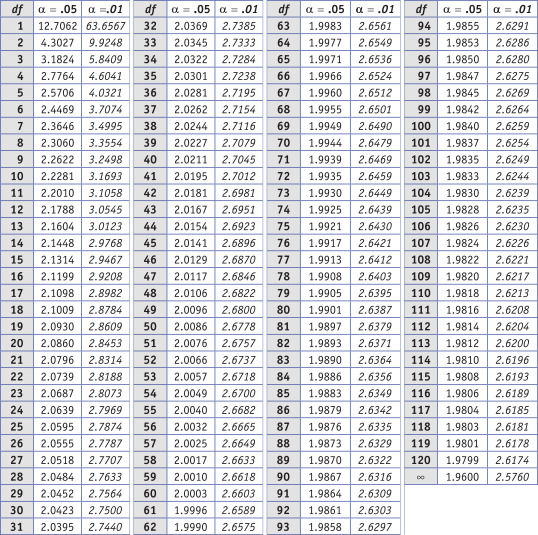
\includegraphics[width=0.7\linewidth]{figs/tabela_t} \end{center}
\end{frame}


\setbeamercovered{transparent}
\begin{frame}
\frametitle{Exemplo 8.3.2}
Uma amostra com 10 observação de uma variável aleatória Normal forneceu média de 5.5 e variância amostral de 4. Deseja-se testar, ao nível de signifiância de 5\%, se a média na população é igual ou menor que 6. Qual a conclusão?
\vspace{1in}
\vspace{1in}

\end{frame}

\setbeamercovered{transparent}
\begin{frame}
\frametitle{Referências bibliográficas}
\printbibliography
\end{frame}

\end{document}